\documentclass[11pt]{article}
\usepackage[utf8]{inputenc}
\usepackage[T1]{fontenc}
\usepackage{amsmath,amssymb,amsthm}
\usepackage{booktabs}
\usepackage{graphicx}
% ---------------------------------------------------------------------------
% LISIBILITE — docs/articles/STYLE_ARTICLES.md §2. A 11pt, une marge de 2,7cm
% donne une ligne de ~90 caracteres, tres au-dessus de l'optimum de lecture
% (65-75) ; et \parskip nul ne separe pas deux paragraphes. Les deux ensemble
% font la page en « bloc gris », quelle que soit la longueur du texte.
% ---------------------------------------------------------------------------
\usepackage[a4paper,textwidth=13.8cm,textheight=22.4cm]{geometry}
\linespread{1.06}
\setlength{\parskip}{.55em plus .15em minus .1em}
\setlength{\parindent}{1.1em}
\usepackage{hyperref}
\usepackage{tikz}
\usetikzlibrary{positioning,arrows.meta,calc}
\tikzset{
  ax/.style={draw=blue!60!black, fill=blue!12, rounded corners=2pt, font=\scriptsize, inner sep=3pt},
  th/.style={draw=blue!60!black, fill=blue!6, rounded corners=2pt, font=\scriptsize, inner sep=3pt},
  goal/.style={draw=green!50!black, fill=green!14, rounded corners=3pt, font=\scriptsize\bfseries, inner sep=3.5pt},
  open/.style={draw, dashed, rounded corners=2pt, font=\scriptsize, inner sep=3pt},
  fl/.style={-{Stealth[length=2mm]}, gray!70},
  gl/.style={-{Stealth[length=2.2mm]}, green!50!black, thick},
}

% ============================================================================
% REGLE D'OR : chaque phrase adossee a un objet du depot.
% Les %% ANCRE: pointent la preuve de chaque section.
% ⚠️ TOUS LES CHIFFRES VIENNENT DE article/dernier_kilometre/MESURES.md, JAMAIS
% de docs/articles/ORGANES.md — celui-ci a derive de huit chiffres sur huit,
% ce que la section sec:drift raconte.
% ============================================================================

\newtheorem{definition}{Definition}
\newtheorem{proposition}{Proposition}
\theoremstyle{remark}\newtheorem{remark}{Remark}

\title{The Last Mile Is Located, Not Crossed:\\
A Kernel-Verified System That Names What It Lacks}

\author{Karl Olivet\thanks{Independent researcher. Contact:
\texttt{karl.olivet@gmail.com}. Code and certified corpus:
\url{https://github.com/Karl-O/bourbaki-theorie-des-ensembles}, at the tag
\texttt{preprint-v1} (\texttt{54ceef5}), which pins the exact state every measurement
reported here was taken on.}}

\date{Preprint --- August 2026}

\begin{document}
\maketitle

\begin{abstract}
A proof search that fails usually returns nothing an engineer can use. We report a
system in which failure returns \emph{the list of formulas that would close the goal if
added to the pool} --- an object, not a status. Around that primitive, twenty-one search
organs accumulated over four months, and the way they accumulated is this paper's main
claim: \textbf{not one came from an architect's intuition}. Each answers a replayable
failure, and the catalogue's most informative column is not what an organ does but which
diagnosis produced it. The trajectory that emerges was not planned. Up to a point the
system \emph{chains} what it is given; then it accepts \emph{proposed} witnesses; then it
\emph{fabricates} one, using Bourbaki's $\tau$ to build a canonical term from the goal
alone --- and the move was forced by a gap the machine itself had written,
$\neg(n = n)$. We also report what the instrument buys elsewhere: given an operation
invented the same morning, $a \oplus b := (a+b)+1$, and two raw laws about $+$, three
organs establish its commutativity in under two seconds and its associativity in
16.43\,s, kernel-closed. Two negative results are the practical payoff. A search that
fails \emph{by growing} --- cost doubling per level, gap count frozen --- is almost never
repaired by more budget; twice out of twice the cause was upstream. And a corpus of
measured traps, fourteen of them, includes a structural law of this kernel that no
amount of design could have anticipated: \emph{terms are opaque, formulas decompose}.
Finally, and least comfortably, we report that our own documentation of this work had
drifted on eight figures out of eight, and what that says about a paper whose thesis is
that one measures rather than decrees.
\end{abstract}

%% ============================================================================
\section{Introduction}
\label{sec:intro}
%% ANCRE: article/dernier_kilometre/PLAN.md (revendications N1-N9) ;
%% MESURES.md pour tout chiffre ; docs/articles/ORGANES.md pour le catalogue.
%% ============================================================================

Ask an automated prover for a theorem it cannot reach and it returns failure: a timeout,
an exhausted budget, an empty list. The information content of that answer is close to
zero, and it is the same answer whether the goal was one lemma away or unreachable in
principle. Everything the search learned on the way --- which subgoals closed, which
hypothesis refused to discharge, which branch died and why --- is discarded with it.

This paper reports a system built on the opposite convention. When its search fails, it
returns \textbf{the set of formulas that would close the goal if they were added to the
pool}. Failure becomes a datum with a shape: not ``no'', but ``no, and here is exactly
what is missing''. We call the component that does this the \emph{need organ}.

\paragraph{The thesis.} The last mile is not crossed in one jump; it is \emph{located}.
A system that fails while producing the exact statement of its lack is worth more than
one that succeeds half the time without knowing why --- because the first can be
improved by construction and the second can only be retried.

\paragraph{What makes the claim testable.} A thesis about how tools should grow is easy
to assert and hard to check. Ours is checkable because the growth is on record. The
organ accreted twenty-one extensions over four months, and for each one the repository
holds the failure that motivated it, in a form that still replays. The catalogue in
Section~\ref{sec:catalogue} therefore carries two columns, and \textbf{the right one ---
``born from which diagnosis'' --- is the load-bearing one}. If the thesis were false,
that column would read like a rationalisation written after the fact. It does not: each
entry names a measurement.

\paragraph{The setting.} Everything runs against an LCF-style kernel implemented over
Bourbaki's own formalism, described in a companion paper. Two of its properties matter
here. The oracle is \emph{exact}: a proposed witness costs at most a dead route, because
the kernel judges, so the system can afford to guess. And the existential quantifier is
not primitive --- $(\exists x)R$ abbreviates a substitution of a $\tau$-term into $R$ ---
which is what later lets an organ \emph{build} a witness out of a goal instead of
searching for one.

\paragraph{Contributions.}
\begin{enumerate}\itemsep2pt
\item \textbf{Failure as a datum} (Section~\ref{sec:organ}). The need organ returns the
obligations that would close the goal, judged by the kernel. 387 lines, protected by 20
tests.
\item \textbf{A growth law, and its evidence} (Section~\ref{sec:catalogue}). Twenty-one
organs, each traceable to a replayable failure. \emph{The tool is deduced from the
diagnosis.} The list is open, not a closed taxonomy.
\item \textbf{A frontier the machine drew} (Section~\ref{sec:frontier}). Chaining,
then accepting proposals, then fabricating. The passage was forced by a gap the system
wrote itself, and the improvement it brought is \emph{not} quantitative: the same number
of goals close, but the shape of the residual gap changes.
\item \textbf{A new algebra in three organs} (Section~\ref{sec:algebra}). Commutativity
of $\oplus$ in under 2\,s, associativity in 16.43\,s, from two raw laws about $+$.
\item \textbf{Two exploitable failure signatures} (Section~\ref{sec:signatures}).
Failing \emph{by growing} indicates an upstream cause, not an insufficient budget; and a
corpus of fourteen measured traps, including a structural law of the kernel.
\item \textbf{Our own drift, measured} (Section~\ref{sec:drift}). The documentation of
this work had gone stale on eight figures out of eight. We report it because a paper
about naming what one lacks owes the reader the case where it stopped doing so.
\end{enumerate}

\paragraph{What this paper does not claim.} No new mathematics: the organs manipulate
statements, and $\oplus$ is a toy whose two laws are immediate corollaries of those of
$+$. No agent architecture: there is no planner, no learned policy, no training loop.
And no generality: twenty-one organs were cut on two subjects, and nothing suggests the
twenty-second problem will not demand five more --- which is, in fact, what the thesis
predicts.

%% ============================================================================
\section{Background: the pool, the route, the gap}
\label{sec:background}
%% ANCRE: outils_ia/decouvertes/besoin.py ; article compagnon pour le noyau.
%% ============================================================================

We summarise only what is needed; the kernel and its trust boundary are the companion
paper's subject.

A \emph{theorem} is a triple: a finite set of hypotheses it still depends on, a
conclusion, and the kernel rule that produced it. It is \emph{closed} when the hypothesis
set is empty. We write $\vdash R$ when the kernel can construct a closed theorem
concluding $R$; every $\vdash$ below is witnessed by an object the repository can rebuild,
never asserted.

A \emph{goal} is a relation to be derived. A \emph{pool} is a finite set of theorems
available to the search. A \emph{route} is one attempted derivation of the goal, and the
\emph{residue} of a route is the hypothesis set of the theorem it actually reached. A
goal typically has several routes, and the same hypothesis may be open on one and closed
on another --- so every verdict below is stated of a hypothesis \emph{on a route}.

\begin{definition}[Gap]\label{def:gap}
A \emph{gap} of a route is a formula which, added to the pool, would let that route close
its goal. The need organ returns, for a failed search, a finite set of gaps.
\end{definition}

The definition is deliberately weak: a gap is not claimed to be minimal, nor necessary,
nor unique. It is what the search would have needed \emph{on the route it took}. That
modesty is what makes it computable and, as Section~\ref{sec:frontier} shows, what makes
its \emph{shape} informative even when its size is not.

%% ============================================================================
\section{The need organ: failure with a shape}
\label{sec:organ}
%% ANCRE: outils_ia/decouvertes/besoin.py (387 l.) ;
%% test_besoin_ferme_et_nomme_ses_manques (4,48 s) ; MESURES.md §1.
%% ============================================================================

The organ takes a goal and a pool and returns either a kernel-certified proof, or a list
of gaps. It is 387 lines of Python and is protected by 20 tests in
\texttt{test\_autonomie.py}; the whole discovery suite is \textbf{42 tests green in
32\,min 50\,s} (Section~\ref{sec:repro}).

Two properties make the returned object useful rather than decorative.

\paragraph{The kernel judges, so guessing is cheap.} Every candidate the organ tries is
submitted to the kernel. A wrong guess produces no theorem and costs one dead route. This
is what makes the proposer architecture of Section~\ref{sec:frontier} affordable: the
system may fabricate a term with no guarantee whatsoever, because nothing downstream will
believe it on trust.

\paragraph{The gaps are the search's own words.} They are not a rendering of the goal for
human consumption; they are formulas the search would have consumed. That distinction is
what makes them actionable --- and it is what makes them a \emph{measurement} of the
distance remaining, rather than an estimate of it.

%% ============================================================================
\section{The catalogue, and its law of growth}
\label{sec:catalogue}
%% ANCRE: docs/articles/ORGANES.md (catalogue) ; MESURES.md §2 pour les ecarts.
%% ⚠️ le catalogue est OUVERT (STYLE_ARTICLES §8) : « 21 identifies », pas un
%% type ferme.
%% ============================================================================

Twenty-one organs have been identified. We write it that way, rather than ``there are
twenty-one'', because the catalogue is a record of encounters and not a partition proved
exhaustive: an organ is added when a failure demands one, so the list grows by meeting
new failures and nothing here bounds how many remain.

\paragraph{The claim.} None of the twenty-one was designed in advance. Each answers a
failure that can be replayed. Four examples, chosen because their diagnoses are of
different kinds:

\begin{center}\small
\begin{tabular}{@{}llp{62mm}@{}}
\toprule
organ & what it does & \textbf{born from which diagnosis} \\
\midrule
v4 & instantiates the pool's $\forall$-facts on the goal
   & the induction hypothesis $S\{n\}$ sat \emph{inert} in the pool: it was present and
     never used \\
v9 & closes a goal $t = t$ by reflexivity
   & measured: a route was carrying $2k = 2k$ as a \emph{gap} \\
v11 & witnesses drawn from the free variables of pool facts
   & v10 extracted head terms only; a defined predicate unfolds and \emph{buries} its
     argument \\
v18 & instantiates a pool law at the moment of applying it
   & v17 matched left-hand sides literally: the pool said $a+b$, the goal contained
     $(a+b)+1$ --- the law was right, its \emph{instance} was missing \\
\bottomrule
\end{tabular}
\end{center}

Read the right-hand column and the left one becomes almost derivable. That asymmetry
\emph{is} the thesis: the tool is deduced from the diagnosis. An architecture designed up
front would have produced a different table --- one whose right column read ``for
generality'' or ``for completeness'', which is what a rationalisation looks like.

\begin{remark}[an organ that vanished]
The catalogue lists a v3, ``merge the gaps of the direct route''. Searching the code for
it returns nothing: it was absorbed or removed, and the catalogue was never updated. We
leave the observation here rather than quietly renumbering, because
Section~\ref{sec:drift} is about exactly this.
\end{remark}

%% ============================================================================
\section{Chaining, proposing, fabricating}
\label{sec:frontier}
%% ANCRE: test_organe_v10_proposeur_par_appartenance ;
%% test_organe_v13_temoin_canonique_fabrique ; PIEGES_MESURES.md §3.
%% ============================================================================

The organ's history has three regimes, and the system passed between them under
pressure rather than by design.

\paragraph{Chaining.} Up to v9, the organ combines what it is given: it instantiates,
detaches, decomposes, recomposes. Faced with an existential goal and a pool naming no
suitable object, it reports the goal itself as its gap --- correct, and useless.

\paragraph{Proposing.} v6 turns the organ into an extension point: witness
\emph{proposers} are functions passed in, and \texttt{besoin.py} does not know what they
are. v10 is the first generic one --- given $(\exists x)\varphi$, the candidates are the
$t$ of pool facts $t \in A$. It knows nothing about any particular problem.

\paragraph{Fabricating.} v10 and v11 \emph{choose} among objects the pool names. When the
pool names none, they are silent. v13 \emph{builds} the canonical witness $\tau_x(\varphi)$
from the goal alone, which Bourbaki's formalism makes a legitimate term rather than a
trick.

\paragraph{What forced the passage.} Not a design review. The system, searching a
decomposition goal with only $\sigma$ proposing $p := n$, wrote as its terminal gap
\[ \neg(n = n) . \]
A gap that cannot be filled by any pool: the search was asking for a contradiction
because it had no way to name a different object. Read as a specification --- and it is
one, since gaps are formulas the search would consume --- it says: \emph{give me a
generator of witnesses}. v6 and then v13 are the answer to that sentence.

\begin{remark}[the improvement is not quantitative]\label{rem:shape}
v13 does not close more goals than v10. Judged on the number of gaps produced, it would
have been discarded. What changes is their \emph{shape}: on a decomposition goal with an
empty pool, v10 returns the intact existential statement, and v13 returns properties of a
named term. The system does not create information --- it changes the form of the
question. Measuring volume would have hidden the only thing that happened.
\end{remark}

\begin{figure}[t]
\centering
\resizebox{\ifdim\width>\linewidth \linewidth\else\width\fi}{!}{%
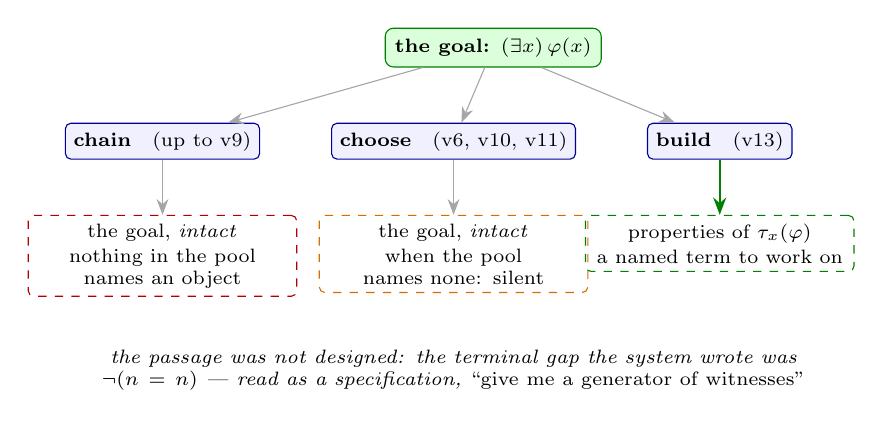
\begin{tikzpicture}[node distance=4mm and 9mm]
%% ---- le meme but existentiel, pose une fois
\node[goal] (but) {the goal: $(\exists x)\,\varphi(x)$};

%% ---- les trois regimes, du plus pauvre au plus riche
\node[th, below=7mm of but, xshift=-42mm] (ch) {\textbf{chain} \; (up to v9)};
\node[th, right=of ch] (pr) {\textbf{choose} \; (v6, v10, v11)};
\node[th, right=of pr] (fa) {\textbf{build} \; (v13)};

%% ---- ce que chacun RETOURNE quand il echoue : c'est la colonne qui compte
\node[open, draw=red!70!black, below=7mm of ch, text width=32mm, align=center] (gch)
  {the goal, \emph{intact}\\[1pt]{\scriptsize nothing in the pool names an object}};
\node[open, draw=orange!85!black, below=7mm of pr, text width=32mm, align=center] (gpr)
  {the goal, \emph{intact}\\[1pt]{\scriptsize when the pool names none: silent}};
\node[open, draw=green!50!black, below=7mm of fa, text width=32mm, align=center] (gfa)
  {properties of $\tau_x(\varphi)$\\[1pt]{\scriptsize a named term to work on}};

\draw[fl] (but) -- (ch);   \draw[fl] (but) -- (pr);   \draw[fl] (but) -- (fa);
\draw[fl] (ch) -- (gch);   \draw[fl] (pr) -- (gpr);   \draw[gl] (fa) -- (gfa);

%% ---- ce qui a FORCE le passage, ecrit par la machine elle-meme
\node[below=6mm of gpr, font=\scriptsize\itshape, text width=96mm, align=center]
  {the passage was not designed: the terminal gap the system wrote was
   $\neg(n = n)$ --- read as a specification, \emph{``give me a generator of
   witnesses''}};
\end{tikzpicture}}
\caption{The three regimes, and what each \emph{returns when it fails} --- the bottom row
is the informative one. Chaining and choosing both hand back the goal untouched; building
hands back properties of a named term. No more goals close
(Remark~\ref{rem:shape}): what changes is the \emph{shape} of the residue.
\textbf{This figure illustrates a distinction, it measures nothing} --- the timings of the
corresponding tests are in Section~\ref{sec:repro}.}
\label{fig:frontiere}
\end{figure}

%% ============================================================================
\section{A freshly invented algebra, in three organs}
\label{sec:algebra}
%% ANCRE: test_organe_v16_congruence_automatique (1,75 s) ;
%% test_organe_v17_chaine_de_reecritures (3,40 s) ;
%% test_organe_v18_associativite_d_une_operation_derivee (16,43 s) ; MESURES.md §3.
%% ============================================================================

The first fifteen organs were all cut on one conjecture. A different question was put on
11 August: is the machinery specific to that subject, or can it approach an algebra it
has never seen?

The protocol is deliberately bare. Define an operation the repository does not know,
\[ a \oplus b \;:=\; (a + b) + 1 , \]
give the system \emph{two raw laws} about $+$ --- iterated associativity, commutativity
--- and nothing else, then ask for the properties of $\oplus$.

\begin{center}\small
\begin{tabular}{@{}llr@{}}
\toprule
goal & closed by & measured \\
\midrule
$a \oplus b = b \oplus a$ & v16 (builds the congruence) & \textbf{1.75\,s} \\
chained rewriting & v17 & 3.40\,s \\
$(a \oplus b) \oplus c = a \oplus (b \oplus c)$ & v17 + v18 & \textbf{16.43\,s} \\
\bottomrule
\end{tabular}
\end{center}

Both results are closed with zero residual hypotheses. The durations are those of the
corresponding tests, and therefore include imports and pool construction --- they bound
the cost from above, which is the direction that matters here.

The associativity chain is worth displaying, because it is what a literal matcher cannot
find and what v18 makes reachable:
\[
\begin{array}{r@{\;}c@{\;}l@{\qquad}l}
((a+b)+1)+c &=& (a+b)+(1+c) & \text{iterated associativity} \\[2pt]
            &=& (a+b)+(c+1) & \text{commutativity, \emph{inside} the right operand} \\[2pt]
            &=& a+(b+(c+1)) & \text{associativity again} \\[2pt]
            &=& a+((b+c)+1) & \text{and again, the other way}
\end{array}
\]
Five steps, none of which matches a pool law \emph{literally}: the pool says $a+b$, the
goal contains $(a+b)+1$. The law was right all along; what was missing was its instance
at the subterm actually encountered. That is v18 in one sentence, and it was found by
looking at a failure, not by reading a textbook on rewriting.

\paragraph{What this does not establish.} $\oplus$ is a toy, and its two laws are
immediate corollaries of those of $+$. Nothing mathematically new is produced. What is
acquired is more modest and more solid: the system can reason equationally about a
structure it has not seen, without being handed the instances. That is a prerequisite,
not a result.

%% ============================================================================
\section{Two exploitable failure signatures}
\label{sec:signatures}
%% ANCRE: docs/journal/ANOMALIES.md (12 aout) ; docs/articles/PIEGES_MESURES.md.
%% ============================================================================

\paragraph{Failing by growing.} The associativity goal above first failed in a way that
looked like an exponential wall: cost doubling with each depth increment, and the number
of gaps frozen at one. The natural reading is ``the problem is hard, raise the budget''.
It was wrong twice out of twice. The actual causes were upstream --- an organ written
twice over, and a bound set by judgement rather than by measurement: the search allowed
three steps where the minimal chain, displayed above, takes five.

We state the resulting rule as a signature, because it is cheap to recognise:

\begin{quote}
A search whose \emph{cost explodes while its gap count stays fixed} is almost never
repaired by more budget. Cost growing means the search is enumerating; gaps not moving
means it is enumerating the wrong thing. Look upstream: at the exploration order, or at a
bound nobody measured.
\end{quote}

The practical consequence adopted since is to \emph{measure the expected chain length
before setting the bound}, which the relevant docstring now carries in figures rather
than in prose.

\paragraph{Traps, paid for.} The repository keeps fourteen traps that were met and paid
for --- not best practices copied from elsewhere. Three carry beyond this project:

\begin{itemize}\itemsep2pt
\item \textbf{The test that never ran.} A conclusion (``proposer v12 closes nothing'')
rested on a call that had silently fallen back to a default for want of a parameter.
\emph{Assert the capability before measuring it}; one line of introspection is enough.
Looking for the reason uncovered the real defect --- proposers were not crossing an
intermediate layer at all.
\item \textbf{The test both branches pass.} To show that fabricating beats choosing, the
trial case was closed by both. A test that both branches pass discriminates nothing; the
case where one fails has to be built on purpose.
\item \textbf{Terms are opaque; formulas decompose.} In this kernel $N(7)$ and
$N(3)+N(4)$ are both $\tau$-terms with a single argument. There is nothing to descend
into: no evaluator can work by walking a term. The only route is reconstruction ---
build the expected term and compare --- which is practical because assemblies are
hashable and equality is $O(1)$. Formulas, by contrast, decompose normally. The boundary
is not a design choice; it is a fact about the substrate, and every tool of this kind has
to be shaped by it.
\end{itemize}

\begin{remark}[the same mistake twice in twenty minutes]
The third trap was met once on terms, then immediately again on predicate recognition,
where the code was navigating by \texttt{.sous[0].sous[1].sous[0]}. The second time,
applying the law just written worked on the first attempt. The generalisation is blunter
than the law: \emph{never assume a structure --- look at it}. Three lines of
introspection settled in seconds what two successive assumptions had cost.
\end{remark}

%% ============================================================================
\section{Our own drift, measured}
\label{sec:drift}
%% ANCRE: MESURES.md §2 (les huit ecarts) ; ORGANES.md et PIEGES_MESURES.md,
%% 10-12 aout, non mis a jour depuis.
%% ============================================================================

This paper's material --- a catalogue of the organs and a corpus of traps --- was written
on 10--12 August. Before drawing a single sentence from it, every figure it contained was
re-measured. \textbf{Eight out of eight had drifted.}

\begin{center}\small
\begin{tabular}{@{}lll@{}}
\toprule
the document says & measured 20 August & nature \\
\midrule
15 tests in \texttt{test\_autonomie.py} & \textbf{20} & tests added, document not updated \\
24 green, 40 min & \textbf{31} in the package; 42 with the corpus, \textbf{32\,min 50} & and \emph{faster} than stated \\
a catalogue of ``nineteen lines'' & \textbf{21} organs & the document contradicts itself \\
\texttt{besoin.py}, 259 lines & \textbf{387} & $+128$ \\
organ v3 & \textbf{no trace in the code} & absorbed or removed, never recorded \\
v16: 0.29\,s & 1.75\,s & \emph{not comparable, see below} \\
v18: 8\,s & 16.43\,s & \emph{idem} \\
v15: 102\,s $\to$ 0\,s & whole test in 2.87\,s & \emph{idem} \\
\bottomrule
\end{tabular}
\end{center}

\paragraph{The reservation that matters.} The last three lines do not show the document to
be wrong. \texttt{pytest --durations} times the \emph{whole test} --- imports, pool
construction, both passes --- whereas the document's figures plainly timed \emph{the organ
call alone}. The two series measure different things, and writing ``the document was
wrong'' would be as sloppy as the drift itself. What is established, and enough for
Section~\ref{sec:algebra}, is an upper bound: under 2\,s, 16.43\,s.

The one claim we withdraw is v15's. The catalogue reports a first pass at 102\,s and a
second at 0\,s --- a striking ratio for a section on capitalisation. The whole test now
runs in 2.87\,s, so that ratio cannot be obtained in the current configuration. The
compounding itself stands: the test asserts that the learned proposer alone, with no
arithmetic access, recloses the goal. \emph{Its magnitude does not.} We report the
assertion and drop the number.

\paragraph{A figure we will not draw.} The material's centrepiece was a curve of the gap
count falling across successive probes, $14 \to 8 \to 6 \to 4 \to 1$, each drop labelled
with the organ that caused it. It comes from a session journal and no script replays it.
It is therefore \textbf{not in this paper}. A curve that cannot be reproduced has no place
in an article whose thesis is that one measures instead of decreeing; opening on it would
have been a refutation in Figure~1.

\paragraph{Why this section exists.} It would have been easy to re-measure quietly, print
the new figures, and say nothing. We report the drift because it is the paper's own thesis
turned on the paper. The claim is that a system should name what it lacks; the
documentation of that system had stopped doing so, and no test caught it --- the kernel
certifies derivations, not the prose written beside them. The same class of defect, at a
different level, is the subject of the companion paper on fidelity.

%% ============================================================================
\section{Reproducibility}
\label{sec:repro}
%% ANCRE: MESURES.md §1 et §3 ; commande unique.
%% ============================================================================

One command, one figure:

\begin{center}
\texttt{python -m pytest outils\_ia/decouvertes/ tests/outils\_ia/corpus/ -q --durations=0}
\end{center}

\textbf{42 tests green in 32\,min 50\,s}, exit 0, at the tag \texttt{preprint-v1}: 20 in
\texttt{test\_autonomie.py}, 9 in the autonomy sub-package, 2 on rediscovered lemmas, and
11 on the two most recent organs, which live in a different tree. Verdicts are read off
the last line of the output file, never off a notification: three ``exit 0'' reports in
this project turned out to be timeouts.

The cost is concentrated in one place. \texttt{test\_euclide\_infinitude} takes
\textbf{1361.87\,s --- 69\% of the whole suite}; every organ test is under 17\,s.
Protecting twenty-one organs is cheap; proving Euclid is not.

%% ============================================================================
\section{Related work}
\label{sec:related}
%% ANCRE: ../references.bib (52 entrees verifiees au 20 aout).
%% ATTENTION : ne rien citer qui ne soit dans le .bib ET verifie a la source.
%% ============================================================================

\emph{[To be completed before freeze, under the discipline stated in the companion paper:
no citation that has not been checked against its source. The repository's bibliography
carries 52 verified entries; the references specific to failure localisation, premise
selection and proof repair are not yet all among them. This section is deliberately left
short rather than padded with unverified citations.]}

Instrumentation work has shown that discarded proof activity can be captured
\cite{ringer2020replica}, and current provers consume failures as training negatives or
repair prompts \cite{first2023baldur,reichel2023proofrepair}. Systems that establish
something by failing to prove --- counterexample search \cite{blanchette2011nitpick},
learned disproof \cite{learningtodisprove2026} --- form a second family, and the
conjecture-generation literature a third \cite{conjecturingsurvey2026}. Our departure is
narrower than any of them: the failure object here is neither a training signal nor a
refutation, but \emph{a list of formulas the search would have consumed}, judged by an
exact kernel. Whether that object is genuinely new we state as the companion paper does
--- semi-decidably: no counterexample found after methodical search, never more.

%% ============================================================================
\section{Limitations}
\label{sec:limitations}
%% ============================================================================

\paragraph{Two subjects, twenty-one organs.} The catalogue was cut on one conjecture and
one toy algebra. Nothing here shows the organs generalise, and the thesis itself predicts
that a genuinely new subject will demand new ones. The honest reading of ``twenty-one'' is
as a record of what two problems required.

\paragraph{The catalogue is open.} We report $21$ identified organs, not a taxonomy proved
exhaustive. Exhibiting a twenty-second is a finite act; proving there is none is not.

\paragraph{Gaps are route-relative and not minimal.} Definition~\ref{def:gap} claims
nothing about minimality or necessity. A gap is what \emph{the route taken} would have
needed; a different route may report a different set, and neither is canonical. The
usefulness demonstrated here is practical, not theoretical.

\paragraph{Durations bound from above.} All timings are test durations including setup,
measured once on one Windows~11 machine (Python~3.13, pytest~9.0.3). They are upper
bounds, not benchmarks, and no averaging over repetitions was done.

\paragraph{Withdrawn and unreproduced claims.} v15's $102\,\mathrm{s} \to 0\,\mathrm{s}$
is withdrawn (Section~\ref{sec:drift}). Two further figures from the material --- a factor
of 100 on term evaluation, and a $24\times$ ratio on the associativity search --- were not
re-run here; they are period measurements, and we do not present them as current.

\paragraph{One mind.} Designed, operated and audited by one person. The re-measurement of
Section~\ref{sec:drift} is a case where self-audit worked --- but it worked because the
material was about to be published, not because a process caught it.

%% ============================================================================
\section{Conclusion}
%% ============================================================================

The system reported here does not solve the problems it is pointed at. What it does is
return, when it fails, a statement of what it would have needed --- and that turned out to
be enough to make the tool grow itself. Twenty-one organs, none designed in advance, each
answering a failure that still replays; a frontier between chaining and fabricating that
the machine crossed under the pressure of a gap it had written; and an algebra invented in
the morning, reasoned about in the afternoon in under twenty seconds.

The two negative results are the ones we would keep. Failing \emph{by growing} is a
signature, and reading it correctly saved a chantier that more budget would not have
opened. And the drift of our own documentation, eight figures out of eight, is the
uncomfortable one: the discipline this paper recommends for a proof search is exactly the
discipline its authors had stopped applying to their own notes.

A prover that says ``no'' teaches nothing. A prover that says ``no, and here is the
formula I lacked'' hands back the only thing that makes the next attempt different from
the last.

\bibliographystyle{plain}
\bibliography{../references}

\end{document}
